\documentclass[10pt,twocolumn]{article}

\usepackage[a4paper,margin=1.8cm,columnsep=0.7cm]{geometry}
\usepackage[T1]{fontenc}
\usepackage{lmodern}
\usepackage{microtype}
\usepackage{amsmath}
\usepackage{graphicx}
\usepackage{booktabs}
\usepackage{xcolor}
\usepackage{caption}
\usepackage{subcaption}
\usepackage{enumitem}
\usepackage{adjustbox}
\usepackage{tikz}
\usetikzlibrary{positioning,arrows.meta,fit,backgrounds,shapes.geometric,calc}
\usepackage[colorlinks=true,linkcolor=teal!60!black,citecolor=teal!60!black,urlcolor=teal!60!black]{hyperref}

\definecolor{read}{HTML}{DCEBF7}
\definecolor{readline}{HTML}{3A78B5}
\definecolor{data}{HTML}{E3F2E6}
\definecolor{dataline}{HTML}{3C8D50}
\definecolor{look}{HTML}{FFF1D6}
\definecolor{lookline}{HTML}{C38A1C}
\definecolor{out}{HTML}{F3E3F1}
\definecolor{outline}{HTML}{94508A}
\definecolor{llm}{HTML}{6B6B6B}

\captionsetup{font=small,labelfont=bf}
\setlist{nosep,leftmargin=1.2em}

\title{\textbf{DeCraft: Generating Believable Decoy Documents\\from a Single Source PDF}}
\author{DeCraft project\\\small Acalvio deception research}
\date{October 2026}

\begin{document}
\maketitle

\begin{abstract}
Decoy documents only work if an intruder believes them. A file that looks generic, or whose numbers
do not add up, is ignored, and a file that copies real figures leaks the very data it is meant to
protect. We describe DeCraft, a pipeline that takes one source PDF and produces a new document with
the source's look and structure but entirely new content. DeCraft separates \emph{proposing} from
\emph{deciding}: language models suggest rules, labels, text and layout fixes, while every rule is
verified against the source numbers in Python, every generated value comes from a seeded generator,
and every printed number is resolved from one canonical dataset. Generation is bounded by explicit
privacy distances and checked by 31 automated gates. On a five-page equity research note with
twelve tables, an offline run finishes in 24\,s, passes all privacy and consistency gates, and passes
29 of 31 gates overall. The two failures are strict read-back layout checks, which show that
matching the source's block geometry, rather than its data or style, is the main open problem.
\end{abstract}

\section{Introduction}

Deception platforms place fake assets (credentials, shares, documents) where only an attacker would
touch them. Documents are attractive bait because intruders go looking for them: a quarterly results
note or a board pack is exactly what an attacker hopes to find. Making such decoys by hand does not
scale, and naive automation produces files that are easy to spot.

A convincing decoy has to meet three requirements at once:
\begin{enumerate}
  \item \textbf{Look.} It must share the publisher's fonts, colours, page grid, chart style and
        section structure.
  \item \textbf{Coherence.} Its data must behave like real data: totals add up, ratios follow their
        formulas, trends and breaks look plausible, and the prose agrees with the tables.
  \item \textbf{Distance.} No confidential value, name or near-identical row from the source may
        survive.
\end{enumerate}
Requirements~2 and~3 pull against each other: the closer the data is to the source, the more
coherent it looks and the more it leaks. DeCraft handles this by learning \emph{structure} from the
source (rules, patterns, layout) and then generating \emph{values} under explicit distance limits.

\section{Method}

Figure~\ref{fig:pipeline} shows the full run. It is a resumable stage machine with seventeen stages
in four phases. Each stage writes its output and a hash of its inputs, so an unchanged stage is
reused on the next run and a failed run resumes where it stopped.

\begin{figure*}[t]
\centering
\begin{adjustbox}{max width=\textwidth}
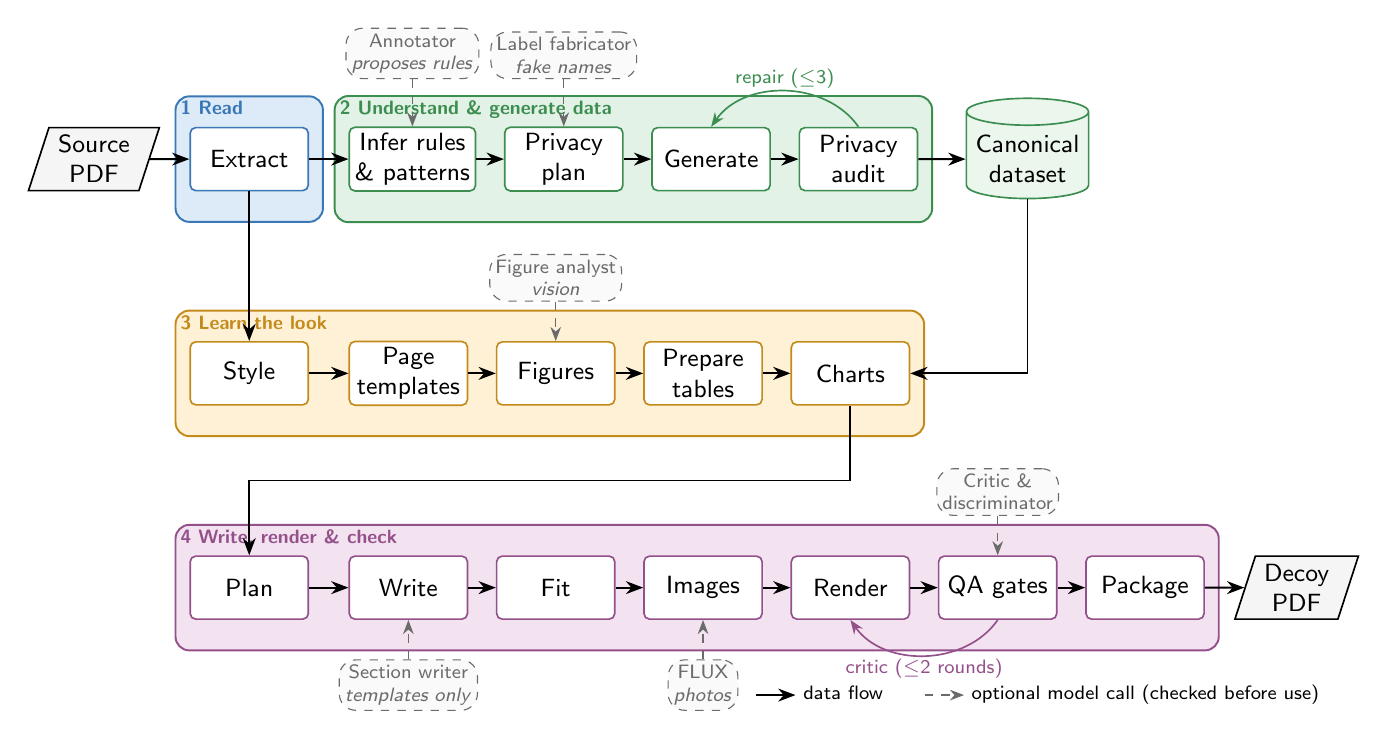
\begin{tikzpicture}[
  font=\sffamily\small,
  stage/.style={draw, rounded corners=2pt, minimum height=8mm, minimum width=15mm, align=center,
                fill=white, line width=0.6pt, inner sep=2pt},
  io/.style={draw, trapezium, trapezium left angle=72, trapezium right angle=108,
             minimum height=8mm, align=center, fill=gray!8, line width=0.6pt, inner sep=1.5pt},
  store/.style={draw, cylinder, shape border rotate=90, aspect=0.22, minimum height=11mm,
                minimum width=15mm, align=center, fill=data!70, draw=dataline, line width=0.6pt},
  llmbox/.style={draw=llm, dashed, rounded corners=6pt, align=center, font=\sffamily\scriptsize,
                 text=llm, fill=gray!4, inner sep=2pt},
  flow/.style={-{Stealth[length=2.2mm]}, line width=0.7pt},
  assist/.style={-{Stealth[length=1.8mm]}, dashed, draw=llm, line width=0.5pt},
  loop/.style={-{Stealth[length=1.8mm]}, line width=0.6pt, draw=#1},
  phase/.style={rounded corners=5pt, inner xsep=5pt, inner ysep=11pt, line width=0.7pt},
  ptitle/.style={font=\sffamily\scriptsize\bfseries, anchor=north west, inner sep=2pt},
  node distance=4.5mm and 3.5mm
]

% ---------- row 1: read, understand, generate
\node[io] (src) {Source\\PDF};
\node[stage, right=5mm of src, draw=readline] (extract) {Extract};
\node[stage, right=5mm of extract, draw=dataline] (infer) {Infer rules\\\& patterns};
\node[stage, right=of infer, draw=dataline] (pplan) {Privacy\\plan};
\node[stage, right=of pplan, draw=dataline] (gen) {Generate};
\node[stage, right=of gen, draw=dataline] (audit) {Privacy\\audit};
\node[store, right=6mm of audit] (cds) {Canonical\\dataset};

% ---------- row 2: the look
\node[stage, below=19mm of extract, draw=lookline] (style) {Style};
\node[stage, right=5mm of style, draw=lookline] (templ) {Page\\templates};
\node[stage, right=of templ, draw=lookline] (figs) {Figures};
\node[stage, right=of figs, draw=lookline] (prep) {Prepare\\tables};
\node[stage, right=of prep, draw=lookline] (charts) {Charts};

% ---------- row 3: write, render, check
\node[stage, below=19mm of style, draw=outline] (plan) {Plan};
\node[stage, right=5mm of plan, draw=outline] (write) {Write};
\node[stage, right=of write, draw=outline] (fit) {Fit};
\node[stage, right=of fit, draw=outline] (images) {Images};
\node[stage, right=of images, draw=outline] (render) {Render};
\node[stage, right=of render, draw=outline] (qa) {QA gates};
\node[stage, right=of qa, draw=outline] (pack) {Package};
\node[io, right=5mm of pack] (decoy) {Decoy\\PDF};

% ---------- phase backgrounds
\begin{scope}[on background layer]
  \node[phase, fill=read, draw=readline, fit=(extract)] (P1) {};
  \node[phase, fill=data, draw=dataline, fit=(infer)(audit)] (P2) {};
  \node[phase, fill=look, draw=lookline, fit=(style)(charts)] (P3) {};
  \node[phase, fill=out, draw=outline, fit=(plan)(pack)] (P4) {};
\end{scope}
\node[ptitle, text=readline] at (P1.north west) {1\,\,Read};
\node[ptitle, text=dataline] at (P2.north west) {2\,\,Understand \& generate data};
\node[ptitle, text=lookline] at (P3.north west) {3\,\,Learn the look};
\node[ptitle, text=outline]  at (P4.north west) {4\,\,Write, render \& check};

% ---------- main flow
\draw[flow] (src) -- (extract);
\draw[flow] (extract) -- (infer);
\draw[flow] (infer) -- (pplan);
\draw[flow] (pplan) -- (gen);
\draw[flow] (gen) -- (audit);
\draw[flow] (audit) -- (cds);
\draw[flow] (extract.south) -- (style.north);
\draw[flow] (style) -- (templ);
\draw[flow] (templ) -- (figs);
\draw[flow] (figs) -- (prep);
\draw[flow] (prep) -- (charts);
\draw[flow] (cds.south) |- (charts.east);
\draw[flow] (charts.south) -- ++(0,-9.5mm) -| (plan.north);
\draw[flow] (plan) -- (write);
\draw[flow] (write) -- (fit);
\draw[flow] (fit) -- (images);
\draw[flow] (images) -- (render);
\draw[flow] (render) -- (qa);
\draw[flow] (qa) -- (pack);
\draw[flow] (pack) -- (decoy);

% ---------- feedback loops
\draw[loop=dataline] (audit.north) to[out=125,in=55]
  node[above, font=\sffamily\scriptsize, text=dataline, inner sep=1pt]{repair ($\le$3)} (gen.north);
\draw[loop=outline] (qa.south) to[out=-125,in=-55]
  node[below, font=\sffamily\scriptsize, text=outline, inner sep=1pt]{critic ($\le$2 rounds)} (render.south);

% ---------- model assistance (proposes only)
\node[llmbox, above=6mm of infer] (ann) {Annotator\\\textit{proposes rules}};
\node[llmbox, above=6mm of pplan] (lab) {Label fabricator\\\textit{fake names}};
\node[llmbox, above=5mm of figs] (fa) {Figure analyst\\\textit{vision}};
\node[llmbox, below=5mm of write] (sw) {Section writer\\\textit{templates only}};
\node[llmbox, below=5mm of images] (flux) {FLUX\\\textit{photos}};
\node[llmbox, above=5mm of qa] (crit) {Critic \&\\discriminator};
\draw[assist] (ann) -- (infer);
\draw[assist] (lab) -- (pplan);
\draw[assist] (fa) -- (figs);
\draw[assist] (sw) -- (write);
\draw[assist] (flux) -- (images);
\draw[assist] (crit) -- (qa);

% ---------- legend
\node[anchor=north east, font=\sffamily\scriptsize, align=left] at ($(decoy.south east)+(0,-7mm)$) {%
  \tikz[baseline=-0.5ex]\draw[flow](0,0)--(5mm,0); data flow\qquad
  \tikz[baseline=-0.5ex]\draw[assist](0,0)--(5mm,0); optional model call (checked before use)};
\end{tikzpicture}
\end{adjustbox}
\caption{The DeCraft run. Solid arrows carry data between stages; dashed boxes are optional model
calls. A model only \emph{proposes}: rules are verified against the source numbers, labels and text
are checked before use, and every stage has a deterministic fallback, so the run completes with no
model at all. All printed numbers come from the canonical dataset.}
\label{fig:pipeline}
\end{figure*}

\subsection{Reading the source}
The source is parsed with Docling (PyMuPDF as fallback) into text blocks, tables and figures with
their bounding boxes. A separate style pass records fonts, text styles, the colour palette and the
page geometry. Results are cached by the PDF's SHA-256, so a cache entry is reused only for the
identical file.

\subsection{Understanding the data}
Each table is graded and each column profiled: type, display scale (\emph{crore}, \emph{million}),
unit, period axis and sensitivity. Rules are then found in two steps. A language model (the
\emph{annotator}) sees the column headers and row labels of statement-like tables and proposes
candidate relations, such as \textit{EBITDA margin = EBITDA / Sales}. Python evaluates every
candidate on the actual rows. A single policy function maps the match rate to a tier and an
enforcement level: at least 95\% of rows within a relative tolerance of 0.5\% makes a rule
\emph{strongly inferred} and \emph{hard}; 80--95\% makes it a soft hypothesis; below 50\% marks it
\emph{contradicted}. Model confidence is deliberately not an input to this policy, so a confident
but wrong proposal can never become a constraint.

Statistical \emph{patterns} are detected separately and are always soft. Trends use Kendall's
$\tau$ with a Theil--Sen slope (at least five points, $|\tau|\ge 0.5$, $p\le 0.10$). Structural
breaks need six points, must persist for two, and must beat the no-break model by 10 BIC points.
Correlations need at least eight rows. A break's cause is kept only if its supporting quote is
actually in the source text.

\subsection{Privacy-aware generation}
Before generating anything, each column gets a privacy decision: regenerate, jitter (for tiny
tables), keep as a period axis, or derive from other columns. The organisation's own name and
branding are kept on purpose, since a decoy has to name its supposed publisher; people's names
and all other labels are replaced by checked fakes.

Generation is a walk over a dependency graph built from the hard rules. Root columns are sampled
from fitted distributions with a copula that keeps strong correlations, trends are re-imposed with
their segment shapes, and derived columns, roll-ups and totals are computed rather than sampled,
so they hold exactly. Identifiers get fresh keys from a disjoint range, and every period label
moves forward one year in its original style (FY24 becomes FY25). The run is seeded and
reproducible.

The privacy audit then checks the result. Every root cell must differ from its source counterpart
by at least 5\%, and every headline fact (totals, growth rates) by at least 10\%. The distance to the
closest source record (a Gower-style mean over columns, with share-of-total columns included so
proportions are compared too) must be at least 0.05. The audit also checks for reused
identifiers, labels and numbers in text, quasi-identifier matches and rare combinations. A
violation triggers a bounded repair, at most three attempts, after which the run fails rather than
ship a leak. The report always states that synthetic data is not automatically anonymous and that
no formal differential-privacy guarantee is claimed.

\subsection{Writing the narrative}
Text is written as \emph{templates}, not prose with numbers in it. A story bible of invented
products, events and initiatives is fixed first, so sections do not contradict each other. The
section writer then produces sentences in which every figure is a placeholder such as
\texttt{\{\{revenue\_growth|pct:1\}\}}, resolved later from the fact store. A draft is rejected if it
contains a literal digit, an unknown key, a typed unit or a \textit{rose}/\textit{fell} that
disagrees with the sign of its fact. This makes it structurally impossible for prose and tables to
disagree. When the model is unavailable, a deterministic writer produces plainer text from the
same facts.

\subsection{Layout, rendering and checks}
Each source page becomes a \emph{page template} of positioned blocks. Safe pages are rendered in
\emph{mirror} mode, with every block at its source position; the rest flow. Charts are redrawn
with Matplotlib in the source palette and chart type, labelled by a vision model where available,
and charts with no backing table are recovered from vector geometry first. Text is fitted to its
box by bounded padding and wording changes, never by changing font sizes. Photos are generated with
FLUX and checked against their caption by the vision model; the source photo is never reused. The
HTML is rendered to PDF with WeasyPrint.

Quality control has three layers. (i) Deterministic gates cover data validity, chart--table
agreement, unresolved placeholders, illegal digits, embedded and locked fonts, source names,
metadata and packaging. (ii) A vision critic compares each output page with its source and may
adjust only whitelisted layout parameters within $\pm$20\%, for at most two rounds; a
discriminator is asked which of the two pages is the published original, in both orders, to cancel
position bias. (iii) A round-trip check feeds the rendered PDF back through DeCraft's own
extractor and compares the recovered blocks with the intended ones (block counts, reading order,
mean IoU, alignment and overlap).

\subsection{Model access}
All model calls go through one gateway that validates each reply against a schema, retries with a
repair hint, and caches every reply under a key that includes the prompt version. Each stage has a
token budget. When a provider reports that its daily quota is used up, the gateway turns that
provider off and the stage falls back to its deterministic path. Because of the cache, any model
run can be replayed exactly and offline.

\section{Results}

\paragraph{Setup.} The source is a five-page equity research note on an Indian power utility with
12 tables, 20 figures and about 3,600 words. The headline run below is fully offline
(\texttt{--no-llm}, seed 42), so it is reproducible without keys; model behaviour was measured in
separate live runs.

\paragraph{Throughput and output.} The offline run takes 24.3\,s end to end, most of it in page
template construction (9.5\,s) and rendering (7.6\,s). It produces a five-page PDF with 2,866 words,
14 narrative sections, 12 regenerated tables, each with a matching chart, and 31 trend patterns
carried over (28 rising, 3 falling). Table~\ref{tab:gates} summarises the gates.

\begin{table}[t]
\centering
\small
\caption{Gate results of the offline run (31 gates).}
\label{tab:gates}
\begin{tabular}{@{}lcc@{}}
\toprule
Gate group & Gates & Passed \\
\midrule
Data validity \& rules            & 4  & 4 \\
Privacy (distance, DCR, reuse)    & 5  & 5 \\
Narrative consistency             & 6  & 6 \\
Fonts, metadata, branding, fit    & 7  & 7 \\
Charts, tables \& OCR             & 4  & 4 \\
Deliverables                      & 1  & 1 \\
Layout read-back                  & 2  & 0 \\
Vision critic / layout model$^{*}$& 2  & 2 \\
\midrule
\textbf{Total}                    & \textbf{31} & \textbf{29} \\
\bottomrule
\end{tabular}
\\[2pt]
\raggedright\footnotesize $^{*}$Not run offline (no vision model, no layout weights); reported as
not blocking.
\end{table}

\paragraph{Privacy and consistency.} All ten privacy checks passed with no violations: no reused
identifiers or labels, every cell and headline beyond its minimum distance, and no generated row
within DCR 0.05 of a source row. Validation found no hard violations and needed no repairs. Its
seven warnings are utility drift: some category shares moved by up to 0.24 and some values left
the widened source range. Every printed number resolved from the fact store, and no
placeholders or stray digits remained.

\paragraph{Layout.} The two failing gates are the strict read-back checks
(Table~\ref{tab:layout}). The page style matches the source closely (Figure~\ref{fig:pages}), and
chart style similarity was 0.98--1.00, but block geometry does not: mean block IoU against the
intended layout is 0.33--0.66 against a 0.9 target, and reading-order similarity is 0.52--0.85
against 0.9. Page~5 also shows one badly misaligned block.

\begin{table}[t]
\centering
\small
\caption{Read-back layout metrics per page (targets: IoU $\ge 0.9$, order $\ge 0.9$).}
\label{tab:layout}
\begin{tabular}{@{}lccccc@{}}
\toprule
Page & 1 & 2 & 3 & 4 & 5 \\
\midrule
Mean block IoU        & 0.37 & 0.48 & 0.33 & 0.43 & 0.66 \\
Reading-order sim.    & 0.85 & 0.67 & 0.52 & 0.75 & 0.80 \\
Text in its box       & 0.91 & 1.00 & 0.00 & 1.00 & 1.00 \\
\bottomrule
\end{tabular}
\end{table}

\begin{figure}[t]
\centering
\begin{subfigure}{0.49\columnwidth}
  \includegraphics[width=\linewidth]{figures/source_p1.png}
  \caption{Source, page 1}
\end{subfigure}\hfill
\begin{subfigure}{0.49\columnwidth}
  \includegraphics[width=\linewidth]{figures/decoy_p1.png}
  \caption{Decoy, page 1 (offline)}
\end{subfigure}
\caption{The header band, palette, fonts, table and chart style carry over; data, periods and
text are new. Offline, the prose is generic and some blocks drift from their source positions.}
\label{fig:pages}
\end{figure}

\paragraph{Model behaviour.} Live runs exposed two provider limits that shaped the design
(Table~\ref{tab:vision}). Llama~3.2 11B Vision answered in free prose despite JSON mode, so every
figure fell back to rule labels, and it rejected any request with two images, which the critic
needs. Llama~4 Scout returned valid JSON on the first attempt for all 13 figures. With the source
and output pages joined side by side into one image, the critic scored page~1 at 8/10, and in a
single trial the discriminator chose the decoy as the published original. Free-tier quotas (200k tokens a day on
the text model, 10,000 neurons a day on Cloudflare) were the practical bottleneck for full runs.

\begin{table}[t]
\centering
\small
\caption{Vision models on the figure-labelling prompt (live, one page).}
\label{tab:vision}
\begin{tabular}{@{}lccc@{}}
\toprule
Model & Valid JSON & 2 images & Neurons \\
\midrule
Llama 3.2 11B Vision   & no  & no (400) & 72 \\
Llama 4 Scout 17B      & yes & yes      & 58 \\
Mistral Small 3.1 24B  & yes & yes      & 42 \\
\bottomrule
\end{tabular}
\end{table}

\section{Discussion and limitations}

The split between proposing and deciding held up in practice: when models failed or ran out of
quota, the run still finished and still passed every privacy and consistency gate. The cost of
running offline is quality, not safety. Without the annotator no rules are found, so totals are
not enforced: on the sample, a shareholding table no longer sums to 100\%. The deterministic writer
is also shorter and more generic than the source, so pages fall below their source word counts.

The weakest part is geometry. Mirror mode places blocks near their source positions, but
table and chart heights driven by new data, together with reflowed text, push blocks off their
boxes, and the read-back extractor then sees merged or split headings and tables. Two gates that
pass offline (the critic and the layout model) pass only because they did not run; they should be
read as ``not measured''. Finally, the privacy checks are distance heuristics and carry no formal
guarantee.

\section{Conclusion}

DeCraft shows that a single source PDF is enough to produce a decoy that keeps the source's style
and statistical shape, keeps every printed number consistent, and stays measurably far from the
source data, with language models used only where their output can be checked. The next steps
are clear from the gates: enforce totals without the model (row and column sums can be found
directly), make layout fitting aware of the read-back metrics, and evaluate realism with people
as well as with a vision discriminator.

\end{document}
